%% ODER: format ==         = "\mathrel{==}"
%% ODER: format /=         = "\neq "
%
%
\makeatletter
\@ifundefined{lhs2tex.lhs2tex.sty.read}%
  {\@namedef{lhs2tex.lhs2tex.sty.read}{}%
   \newcommand\SkipToFmtEnd{}%
   \newcommand\EndFmtInput{}%
   \long\def\SkipToFmtEnd#1\EndFmtInput{}%
  }\SkipToFmtEnd

\newcommand\ReadOnlyOnce[1]{\@ifundefined{#1}{\@namedef{#1}{}}\SkipToFmtEnd}
\DeclareFontFamily{OT1}{cmtex}{}
\DeclareFontShape{OT1}{cmtex}{m}{n}
  {<5><6><7><8>cmtex8
   <9>cmtex9
   <10><10.95><12><14.4><17.28><20.74><24.88>cmtex10}{}
\DeclareFontShape{OT1}{cmtex}{m}{it}
  {<-> ssub * cmtt/m/it}{}
\newcommand{\texfamily}{\fontfamily{cmtex}\selectfont}
\DeclareFontShape{OT1}{cmtt}{bx}{n}
  {<5><6><7><8>cmtt8
   <9>cmbtt9
   <10><10.95><12><14.4><17.28><20.74><24.88>cmbtt10}{}
\DeclareFontShape{OT1}{cmtex}{bx}{n}
  {<-> ssub * cmtt/bx/n}{}
\newcommand{\tex}[1]{\text{\texfamily#1}}	% NEU

\newcommand{\Sp}{\hskip.33334em\relax}


\newcommand{\Conid}[1]{\mathit{#1}}
\newcommand{\Varid}[1]{\mathit{#1}}
\newcommand{\anonymous}{\kern0.06em \vbox{\hrule\@width.5em}}
\newcommand{\plus}{\mathbin{+\!\!\!+}}
\newcommand{\bind}{\mathbin{>\!\!\!>\mkern-6.7mu=}}
\newcommand{\rbind}{\mathbin{=\mkern-6.7mu<\!\!\!<}}% suggested by Neil Mitchell
\newcommand{\sequ}{\mathbin{>\!\!\!>}}
\renewcommand{\leq}{\leqslant}
\renewcommand{\geq}{\geqslant}

%mathindent has to be defined
\@ifundefined{mathindent}%
  {\newdimen\mathindent\mathindent\leftmargini}%
  {}%

\def\resethooks{%
  \global\let\SaveRestoreHook\empty
  \global\let\ColumnHook\empty}
\newcommand*{\savecolumns}[1][default]%
  {\g@addto@macro\SaveRestoreHook{\savecolumns[#1]}}
\newcommand*{\restorecolumns}[1][default]%
  {\g@addto@macro\SaveRestoreHook{\restorecolumns[#1]}}
\newcommand*{\aligncolumn}[2]%
  {\g@addto@macro\ColumnHook{\column{#1}{#2}}}

\resethooks

\newcommand{\onelinecommentchars}{\quad-{}- }
\newcommand{\commentbeginchars}{\enskip\{-}
\newcommand{\commentendchars}{-\}\enskip}

\newcommand{\visiblecomments}{%
  \let\onelinecomment=\onelinecommentchars
  \let\commentbegin=\commentbeginchars
  \let\commentend=\commentendchars}

\newcommand{\invisiblecomments}{%
  \let\onelinecomment=\empty
  \let\commentbegin=\empty
  \let\commentend=\empty}

\visiblecomments

\newlength{\blanklineskip}
\setlength{\blanklineskip}{0.66084ex}

\newcommand{\hsindent}[1]{\quad}% default is fixed indentation
\let\hspre\empty
\let\hspost\empty
\newcommand{\NB}{\textbf{NB}}
\newcommand{\Todo}[1]{$\langle$\textbf{To do:}~#1$\rangle$}

\EndFmtInput
\makeatother
%
%
%
%
%
%
% This package provides two environments suitable to take the place
% of hscode, called "plainhscode" and "arrayhscode". 
%
% The plain environment surrounds each code block by vertical space,
% and it uses \abovedisplayskip and \belowdisplayskip to get spacing
% similar to formulas. Note that if these dimensions are changed,
% the spacing around displayed math formulas changes as well.
% All code is indented using \leftskip.
%
% Changed 19.08.2004 to reflect changes in colorcode. Should work with
% CodeGroup.sty.
%
\ReadOnlyOnce{polycode.fmt}%
\makeatletter

\newcommand{\hsnewpar}[1]%
  {{\parskip=0pt\parindent=0pt\par\vskip #1\noindent}}

% can be used, for instance, to redefine the code size, by setting the
% command to \small or something alike
\newcommand{\hscodestyle}{}

% The command \sethscode can be used to switch the code formatting
% behaviour by mapping the hscode environment in the subst directive
% to a new LaTeX environment.

\newcommand{\sethscode}[1]%
  {\expandafter\let\expandafter\hscode\csname #1\endcsname
   \expandafter\let\expandafter\endhscode\csname end#1\endcsname}

% "compatibility" mode restores the non-polycode.fmt layout.

\newenvironment{compathscode}%
  {\par\noindent
   \advance\leftskip\mathindent
   \hscodestyle
   \let\\=\@normalcr
   \let\hspre\(\let\hspost\)%
   \pboxed}%
  {\endpboxed\)%
   \par\noindent
   \ignorespacesafterend}

\newcommand{\compaths}{\sethscode{compathscode}}

% "plain" mode is the proposed default.
% It should now work with \centering.
% This required some changes. The old version
% is still available for reference as oldplainhscode.

\newenvironment{plainhscode}%
  {\hsnewpar\abovedisplayskip
   \advance\leftskip\mathindent
   \hscodestyle
   \let\hspre\(\let\hspost\)%
   \pboxed}%
  {\endpboxed%
   \hsnewpar\belowdisplayskip
   \ignorespacesafterend}

\newenvironment{oldplainhscode}%
  {\hsnewpar\abovedisplayskip
   \advance\leftskip\mathindent
   \hscodestyle
   \let\\=\@normalcr
   \(\pboxed}%
  {\endpboxed\)%
   \hsnewpar\belowdisplayskip
   \ignorespacesafterend}

% Here, we make plainhscode the default environment.

\newcommand{\plainhs}{\sethscode{plainhscode}}
\newcommand{\oldplainhs}{\sethscode{oldplainhscode}}
\plainhs

% The arrayhscode is like plain, but makes use of polytable's
% parray environment which disallows page breaks in code blocks.

\newenvironment{arrayhscode}%
  {\hsnewpar\abovedisplayskip
   \advance\leftskip\mathindent
   \hscodestyle
   \let\\=\@normalcr
   \(\parray}%
  {\endparray\)%
   \hsnewpar\belowdisplayskip
   \ignorespacesafterend}

\newcommand{\arrayhs}{\sethscode{arrayhscode}}

% The mathhscode environment also makes use of polytable's parray 
% environment. It is supposed to be used only inside math mode 
% (I used it to typeset the type rules in my thesis).

\newenvironment{mathhscode}%
  {\parray}{\endparray}

\newcommand{\mathhs}{\sethscode{mathhscode}}

% texths is similar to mathhs, but works in text mode.

\newenvironment{texthscode}%
  {\(\parray}{\endparray\)}

\newcommand{\texths}{\sethscode{texthscode}}

% The framed environment places code in a framed box.

\def\codeframewidth{\arrayrulewidth}

\newenvironment{framedhscode}%
  {\parskip=\abovedisplayskip\par\noindent
   \hscodestyle
   \arrayrulewidth=\codeframewidth
   \tabular{@{}|p{\linewidth-2\arraycolsep-2\arrayrulewidth-2pt}|@{}}%
   \hline\framedhslinecorrect\\{-1.5ex}%
   \let\endoflinesave=\\
   \let\\=\@normalcr
   \(\pboxed}%
  {\endpboxed\)%
   \framedhslinecorrect\endoflinesave{.5ex}\hline
   \endtabular
   \parskip=\belowdisplayskip\par\noindent
   \ignorespacesafterend}

\newcommand{\framedhslinecorrect}[2]%
  {#1[#2]}

\newcommand{\framedhs}{\sethscode{framedhscode}}

% The inlinehscode environment is an experimental environment
% that can be used to typeset displayed code inline.

\newenvironment{inlinehscode}%
  {\(\def\column##1##2{}%
   \let\>\undefined\let\<\undefined\let\\\undefined
   \newcommand\>[1][]{}\newcommand\<[1][]{}\newcommand\\[1][]{}%
   \def\fromto##1##2##3{##3}%
   \def\nextline{}}{\) }%

\newcommand{\inlinehs}{\sethscode{inlinehscode}}

% The joincode environment is a separate environment that
% can be used to surround and thereby connect multiple code
% blocks.

\newenvironment{joincode}%
  {\let\orighscode=\hscode
   \let\origendhscode=\endhscode
   \def\endhscode{\def\hscode{\endgroup\def\@currenvir{hscode}\\}\begingroup}
   %\let\SaveRestoreHook=\empty
   %\let\ColumnHook=\empty
   %\let\resethooks=\empty
   \orighscode\def\hscode{\endgroup\def\@currenvir{hscode}}}%
  {\origendhscode
   \global\let\hscode=\orighscode
   \global\let\endhscode=\origendhscode}%

\makeatother
\EndFmtInput
%

\chapter{Syntax}
\todo[inline]{Rewrite this to only be about the syntax}
Going back to seeing hardware components as computational units \todo{As in chapter x? -> need ref} we can again take a look at what we are trying to \textit{do} and separating this from other information, essentially removing spatial reasoning from the body of the function.
Before doing so, we can formulate a different semantical view on memory elements.
Instead of seeing registers as memory elements which need to hold data we can see registers as elements which transfer a value which is valid in one clockcycle to the next clockcycle. 
Without such an element the value simply will not exist anymore in the next clockcycle.
A register therefor introduces \textit{temporal} behaviour.
If we try to formulate the behaviour of a register in a streaming language we could formulate it as\footnote{\ensuremath{\sigma_1} is a delay of 1 cycle}:
\begin{texexp}{text only}
\begin{hscode}\SaveRestoreHook
\column{B}{@{}>{\hspre}l<{\hspost}@{}}%
\column{E}{@{}>{\hspre}l<{\hspost}@{}}%
\>[B]{}\Varid{register}\mathbin{::}\Varid{a}\to \Varid{a}{}\<[E]%
\\
\>[B]{}\Varid{register}\mathrel{=}\sigma_1{}\<[E]%
\ColumnHook
\end{hscode}\resethooks
\end{texexp}

In this case it is rather unobstrusive, but in the case of the circuit from figure \ref{fig:mul32add} it is already harder to figure out the temporal behaviour from the description in code snippet \ref{code:mul32add}.
\begin{figure}
\centering
\footnotesize
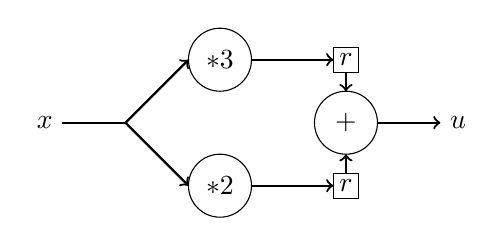
\begin{tikzpicture}[scale=0.8]
\draw (5,0) circle (0.5cm);
\draw (5,0) node { $*2$ };
\draw (5,2) circle (0.5cm);
\draw (5,2) node { $*3$ };
\draw[->,thick] (5.5,0) -- (6.8,0);
\draw[->,thick] (7,0.2) -- (7,0.5);
\draw[->,thick] (5.5,2) -- (6.8,2);
\draw[->,thick] (7,1.8) -- (7,1.5);
\draw(7,1) circle (0.5cm);

\draw (6.8,1.8) rectangle +(0.4,0.4);
\draw (7,2) node { $r$ };
\draw (7,0) node { $r$ };
\draw (6.8,-0.2) rectangle +(0.4,0.4);

\draw (7,1) node { $+$ };
\draw[->,thick] (7.5,1) -- (8.5,1);
\draw[-,thick] (2.5,1) -- (3.5,1);
\draw[->,thick] (3.5,1) -- (4.5,2);
\draw[->,thick] (3.5,1) -- (4.5,0);
\draw (2.5,1) node[left] { $x$ };
\draw (8.5,1) node[right] { $u$ };
\end{tikzpicture}
%%\caption{A specific multiply and add} \label{fig:mul32add}
\end{figure}

\begin{texexptitled}[text only,float]{Definition for a specific multiply and add}{code:mul32add}
\begin{hscode}\SaveRestoreHook
\column{B}{@{}>{\hspre}l<{\hspost}@{}}%
\column{5}{@{}>{\hspre}l<{\hspost}@{}}%
\column{17}{@{}>{\hspre}l<{\hspost}@{}}%
\column{E}{@{}>{\hspre}l<{\hspost}@{}}%
\>[B]{}\Varid{simple}\mathbin{::}\Conid{Num}\;\Varid{a}\Rightarrow \vec a\to \vec a{}\<[E]%
\\
\>[B]{}\Varid{simple}\;\Varid{x}\mathrel{=}\Varid{y}\mathbin{+}\Varid{z}{}\<[E]%
\\
\>[B]{}\hsindent{5}{}\<[5]%
\>[5]{}\mathbf{where}\;{}\<[17]%
\>[17]{}\Varid{y}\mathrel{=}\sigma_1\;(\Varid{x}\mathbin{*}\mathrm{3}){}\<[E]%
\\
\>[17]{}\Varid{z}\mathrel{=}\sigma_1\;(\Varid{x}\mathbin{*}\mathrm{2}){}\<[E]%
\ColumnHook
\end{hscode}\resethooks
%%\caption{A definition for a specific multiply and add} \label{code:mul32add}
\end{texexptitled}
, where we need to figure out what is delayed in which portion of the definition.
According to some document on the Lustre language \todo{reference}, we can view functional relationships over data flows as time invariant.
If we try to break it down to the essence we can define a computation in three parts:
\begin{itemize}
\item What kind of data are we dealing with 
\item When is the data available
\item What do we do with the data
\end{itemize}

Where traditional languages combine the latter two in the body of the function, we will show that combining the first two in the type signature is not only an option, but produces elegant representations of hardware structures.

\section{Semantics}
\subsection{Chronological Functions}
Before defining the actual syntactical rules we first need to define a programming model.
To create an elegant system, syntax must follow semantics and syntax must be able to concisely and accurately capture the semantics of a language.
The basic unit of computation used in here are \textit{chronological functions}.
A chronological function has the ability to introduce a delay (i.e. latency).
Like mentioned before, this is not a new idea, since other languages already have the ability to introduce a delay.
However, the difference with our approach is:
\begin{inparaenum}
\item we introduce delays at the type level;
\item we allow indexing of \textit{abstract} moments in time.
\end{inparaenum}
To do this we introduce the \ensuremath{\Delta_x} operation, which is simply the \ensuremath{\sigma_x} operator as mentioned before but at the type level.
The \ensuremath{\sigma_x} operation can then be expressed as a identity function which includes the \ensuremath{\Delta_x} operation at the type level and may be polymorph in the type of expected data, like the \ensuremath{\Varid{id}\mathbin{::}\Varid{a}\to \Varid{a}} function in Haskell.
Since real systems have to be causal, we can only move values forward in time.

To drive this intuition of chronological functions home we can map a single structural representation of a chronological function over a stream of values.
Take for instance the rather simple representation of adding two temporally shifted values as shown in figure \ref{fig:addtwotemp}.
\begin{figure}
\centering
\footnotesize
\begin{tikzpicture}[scale=0.8]
\draw[->] (0,-0.5) -- (3,-0.5);
\draw[-] (4,-0.5) -- (5,-0.5);
\draw[->] (5,-0.5) -- (5,-1.5);
\draw (0,-0.5) node[left] {$in_1$};
\draw[->] (0,-2) -- (4.5,-2);
\draw (0,-2) node[left] {$in_2$};
\draw[->] (5.5,-2) -- (6.5,-2);
\draw (6.5,-2) node[right] {$out$};

\draw (3,-1) rectangle (4,0);
\draw (3.2,-1) -- (3.5,-0.7);
\draw (3.8,-1) -- (3.5,-0.7);

\draw (5,-2) circle (0.5);
\draw (5,-2) node {$+$};
\end{tikzpicture}
%%\caption{Adding temporally shifted values} \label{fig:addtwotemp}
\end{figure}
If we define $\vec{in1} = (in1_0,in1_1,\ldots,in1_n)$ and $\vec{in2} = (in2_0,in2_1,\ldots in2_m)$ then the result would be $\vec{out} = (in1_0 + \bot,in1_1 + in2_0, \ldots in1_l,in2_{l-1})$ where $l = min(m,n)$.
If we map this structural representation over a stream of values, we can unfold the structure and reveal its temporal behaviour as shown in figure \ref{fig:addtwotemp2}.
\begin{figure}
\centering
\footnotesize
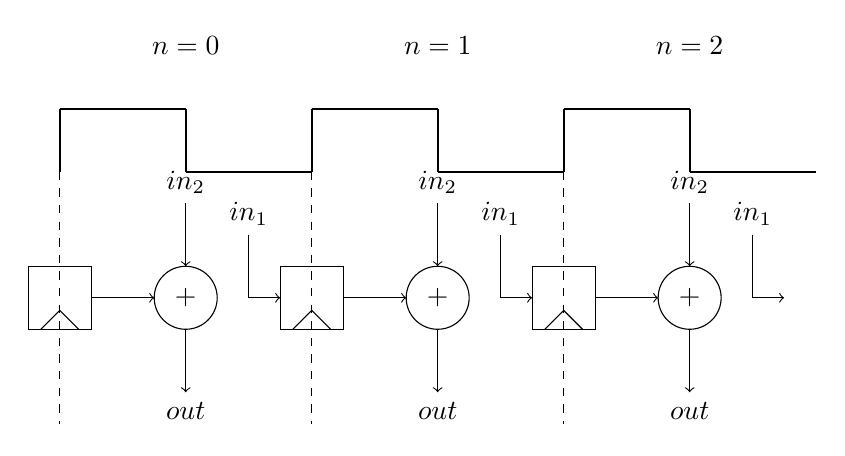
\begin{tikzpicture}[scale=0.8]
\foreach \c/\t in {0/0,4/1,8/2} {
    \draw (2+\c,2) node {$n=\t$};
    \draw[-,thick] (0+\c,1) -- (0+\c,0);
    \draw[-,thick] (0+\c,1) -- (2+\c,1);
    \draw[-,thick] (2+\c,1) -- (2+\c,0);
    \draw[-,thick] (2+\c,0) -- (4+\c,0);

    \draw[dashed] (0+\c,0) -- (0+\c,-4);

    \draw (-0.5+\c,-2.5) rectangle (0.5+\c,-1.5);
    \draw (-0.3+\c,-2.5) -- (0+\c,-2.2);
    \draw (0.3+\c,-2.5) -- (0+\c,-2.2);

    \draw (2+\c,-2) circle (0.5);
    \draw (2+\c,-2) node {$+$};

    \draw[->] (0.5+\c,-2) -- (1.5+\c,-2);

    \draw[->] (2+\c,-0.5) -- (2+\c,-1.5);
    \draw[-] (3+\c,-1) -- (3+\c,-2);
    \draw[->] (3+\c,-2) -- (3.5+\c,-2);
    \draw (2+\c,-0.5) node[above] {$in_2$};
    \draw (3+\c,-1) node[above] {$in_1$};

    \draw[->] (2+\c,-2.5) -- (2+\c,-3.5);
    \draw (2+\c,-3.5) node[below] {$out$};
}
\end{tikzpicture}
%%\caption{Temporal perspective of adding temporally shifted values} \label{fig:addtwotemp2}
\end{figure}
Using this perspective we can clearly see that there is a temporal relation between both inputs and the output.
We can introduce a time quantifier to capture this temporal relation at the type level.
We introduce \ensuremath{\psi. n.\;\Conid{T}}, where \ensuremath{\Conid{T}} is some valid type which references this time quantifier and may apply a certain \ensuremath{\Delta_x} to \ensuremath{\Varid{n}}.
The structure type of the above function would then be: 
\begin{texexp}{text only}
\begin{hscode}\SaveRestoreHook
\column{B}{@{}>{\hspre}l<{\hspost}@{}}%
\column{E}{@{}>{\hspre}l<{\hspost}@{}}%
\>[B]{}\Varid{foo}\mathbin{::}\psi. n.\;\Varid{a}\;\Varid{n}\to \Varid{a}\;(\Delta_1\;\Varid{n})\to \Varid{a}\;(\Delta_1\;\Varid{n}){}\<[E]%
\\
\>[B]{}\Varid{foo}\;\Varid{x}\;\Varid{y}\mathrel{=}\Varid{x}\mathbin{+}\Varid{y}{}\<[E]%
\ColumnHook
\end{hscode}\resethooks
\end{texexp}
where \ensuremath{\Varid{a}} is a datatype which allows numerical operations.

While we have captured the essence of the computation we are trying te express, we have not been able to do this elegantly.
Firstly, the time quantifier does not have to be explicitly declared, since we can deduce from the ground types alone that there are certain quantifiers.
Secondly, the \ensuremath{\Delta_x} construct is hard to represent using ASCII values.
Therefor we introduce a syntactic style, shown in code snippet \ref{code:chronostyle} which only needs ASCII values and matches well with the semantics of chronological functions.
\begin{texexptitled}[text only,float]{Definition for a specific multiply and add}{code:mul32add}
\begin{hscode}\SaveRestoreHook
\column{B}{@{}>{\hspre}l<{\hspost}@{}}%
\column{E}{@{}>{\hspre}l<{\hspost}@{}}%
\>[B]{}\Varid{foo}\mathbin{::}\Varid{a}\langle\Varid{n}\rangle\to \Varid{a}\langle\Varid{n}\mathbin{+}\mathrm{1}\rangle\to \Varid{a}\langle\Varid{n}\mathbin{+}\mathrm{1}\rangle{}\<[E]%
\\
\>[B]{}\Varid{foo}\;\Varid{x}\;\Varid{y}\mathrel{=}\Varid{x}\mathbin{+}\Varid{y}{}\<[E]%
\ColumnHook
\end{hscode}\resethooks
%\caption{Introduction of syntactic style for chronological functions} \label{code:chronostyle}
\end{texexptitled}
It is important to realize that $n$ is still a unbound time quantifier, which is only in scope for this specific function.
If we were to define another function which references $n$, then this is a distinctly different $n$.
Defining a register, if we want to explicitly use memory elements in the function body, can be easily done as well, as shown in code snippet \ref{code:chronoreg}.
\begin{texexptitled}[text only,float]{Definition for a specific multiply and add}{code:mul32add}
\begin{hscode}\SaveRestoreHook
\column{B}{@{}>{\hspre}l<{\hspost}@{}}%
\column{E}{@{}>{\hspre}l<{\hspost}@{}}%
\>[B]{}\Varid{register}\mathbin{::}\Varid{a}\langle\Varid{n}\rangle\to \Varid{a}\langle\Varid{n}\mathbin{+}\mathrm{1}\rangle{}\<[E]%
\\
\>[B]{}\Varid{register}\;\Varid{x}\mathrel{=}\Varid{x}{}\<[E]%
\ColumnHook
\end{hscode}\resethooks
%\caption{Register representation using chronological functions} \label{code:chronoreg}
\end{texexptitled}
As can be seen from the small examples, we are able to introduce delays in function types as we see fit.
The syntax \ensuremath{\langle\Varid{n}\mathbin{+}\Varid{a}\rangle} here really just provides a clean and simple interface to the time tags as proposed earlier.\todo{expand on this}

\subsection{Non-streaming functions}
So far we have only introduced chronological functions which allow streaming. 
However, sometimes we cannot define a component in terms of streaming values, at least not directly.
For instance, a component may induce a latency of 2 clockcycles, but may not be able to process \textit{any} inputs during its computation.
What we want to express here is basically a component with the following signature:
\begin{texexp}{text only}
\begin{hscode}\SaveRestoreHook
\column{B}{@{}>{\hspre}l<{\hspost}@{}}%
\column{E}{@{}>{\hspre}l<{\hspost}@{}}%
\>[B]{}\Varid{waitForMe}\mathbin{::}\Varid{a}\langle\Varid{n}\rangle\to \Varid{a}\langle\Varid{n}\mathbin{+}\mathrm{2}\rangle{}\<[E]%
\\
\>[B]{}\Varid{waitForMe}\mathrel{=}\Varid{id}{}\<[E]%
\ColumnHook
\end{hscode}\resethooks
\end{texexp}

From the model described earlier, especially using figure \todo{ref naar figuur hier die het model beschrijft} , we interpret this as a streaming function.
However, this is not really a streaming function but an operation which operates at a \textit{lower} clockspeed. 
For every 2 cycles this component should produce exactly one value.
Suppose we have an input signal $\vec{s} = (s_0,s_1,\ldots,s_n)$, then \ensuremath{\Varid{waitForMe}} $\vec{s} = (s_0,s_2,\ldots s_n)$, which basically indicates this is a result which is synchronized by a clock which has half the frequency of the clock it was originally in.
Using these results we can write down what we want, provided we allow multiplication as well as addition in time tags, as shown in code snippet \ref{code:waitforme}.
\begin{texexptitled}[text only,float]{Definition for a specific multiply and add}{code:mul32add}
\begin{hscode}\SaveRestoreHook
\column{B}{@{}>{\hspre}l<{\hspost}@{}}%
\column{E}{@{}>{\hspre}l<{\hspost}@{}}%
\>[B]{}\Varid{waitForMe}\mathbin{::}\Varid{a}\langle\Varid{n}\rangle\to \Varid{a}\langle\Varid{n}\mathbin{*}\mathrm{2}\rangle{}\<[E]%
\\
\>[B]{}\Varid{waitForMe}\mathrel{=}\Varid{id}{}\<[E]%
\ColumnHook
\end{hscode}\resethooks
%\caption{Mapping a signal with a fast clock to a signal with a slower clock}\label{code:waitforme}
\end{texexptitled}
If we unfold this in time we can see how this makes sense in terms of different clock frequencies:
\begin{figure}[H]
\centering
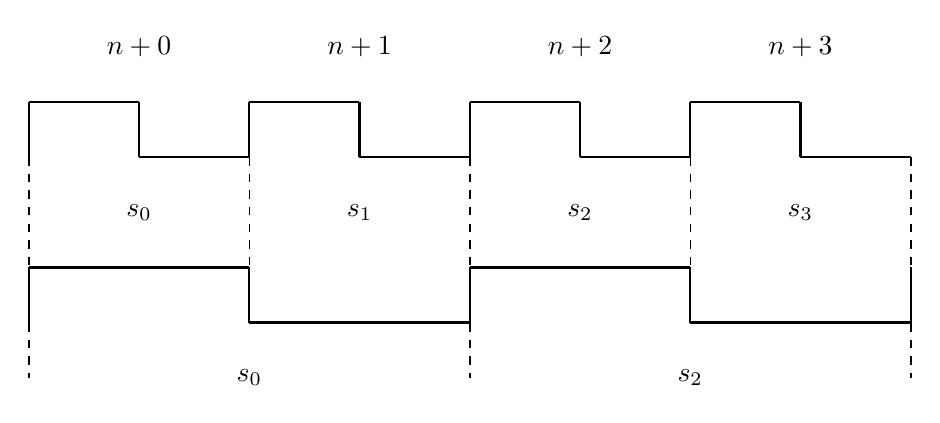
\begin{tikzpicture}[scale=0.7]
\foreach \c/\t in {0/0,4/1,8/2,12/3} {
    \draw (2+\c,2) node {$n+\t$};
    \draw[-,thick] (0+\c,1) -- (0+\c,0);
    \draw[-,thick] (0+\c,1) -- (2+\c,1);
    \draw[-,thick] (2+\c,1) -- (2+\c,0);
    \draw[-,thick] (2+\c,0) -- (4+\c,0);

    \draw[dashed] (0+\c,0) -- (0+\c,-2);

    \draw (2+\c,-1) node {$s_\t$};
}
\foreach \c/\t in {0/0,8/2} {
    \draw[-,thick] (0+\c,-2) -- (0+\c,-3);
    \draw[-,thick] (0+\c,-2) -- (4+\c,-2);
    \draw[-,thick] (4+\c,-2) -- (4+\c,-3);
    \draw[-,thick] (4+\c,-3) -- (8+\c,-3);
    \draw[dashed,thick] (0+\c,0) -- (0+\c,-4);
    \draw (4+\c,-4) node {$s_\t$};
}

\draw[-,thick] (16,-2) -- (16,-3);
\draw[dashed,thick] (16,0) -- (16,-4);
\end{tikzpicture}
%\caption{Temporal mapping of a fast clock to a slow clock} \label{fig:waitforme}
\end{figure}

Sometimes we would like to be able to do the inverse however, which can be specified as shown by code snippet \ref{code:keepup}.
\begin{texexptitled}[text only,float]{Definition for a specific multiply and add}{code:mul32add}
\begin{hscode}\SaveRestoreHook
\column{B}{@{}>{\hspre}l<{\hspost}@{}}%
\column{E}{@{}>{\hspre}l<{\hspost}@{}}%
\>[B]{}\Varid{keepUp}\mathbin{::}\Varid{a}\langle\mathrm{2}\mathbin{*}\Varid{n}\rangle\to \Varid{a}\langle\Varid{n},\Varid{n}\mathbin{+}\mathrm{1}\rangle{}\<[E]%
\\
\>[B]{}\Varid{keepUp}\;\Varid{x}\mathrel{=}\langle\Varid{x},\Varid{x}\rangle{}\<[E]%
\ColumnHook
\end{hscode}\resethooks
%\caption{Mapping a signal with a fast clock to a signal with a slower clock}\label{code:keepup}
\end{texexptitled}
The temporal perspective is slightly different as a result, shown in figure \ref{fig:keepup}.
The semantics of \ensuremath{\langle\Varid{x},\Varid{x}\rangle} might not be clear from this snippet alone. 
Later in \todo{referentie naar sugar} we will expand on this syntax some more, but for the purpose of explanation we will quickly define it here as well.
The $\langle x_1,x_2,\ldots,x_m \rangle$ can be seen as the inverse of sampling a stream of values; it injects the value $x_1$ first, then value $x_2$, et cetera. 
This of course assumes the length of $m$ here corresponds with the number of elements in \ensuremath{\Varid{a}\langle\Varid{n},\Varid{n}\mathbin{+}\mathrm{1},\mathbin{...},\Varid{n}\mathbin{+}\Varid{m}\rangle}, which is introduced through the type signature. 
\begin{figure}[H]
\centering
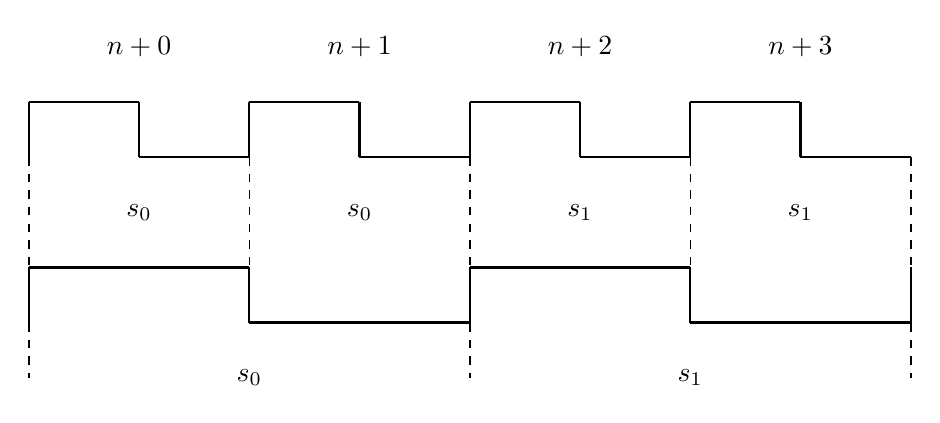
\begin{tikzpicture}[scale=0.7]
\foreach \c/\t/\i in {0/0/0,4/1/0,8/2/1,12/3/1} {
    \draw (2+\c,2) node {$n+\t$};
    \draw[-,thick] (0+\c,1) -- (0+\c,0);
    \draw[-,thick] (0+\c,1) -- (2+\c,1);
    \draw[-,thick] (2+\c,1) -- (2+\c,0);
    \draw[-,thick] (2+\c,0) -- (4+\c,0);

    \draw[dashed] (0+\c,0) -- (0+\c,-2);

    \draw (2+\c,-1) node {$s_\i$};
}
\foreach \c/\t in {0/0,8/1} {
    \draw[-,thick] (0+\c,-2) -- (0+\c,-3);
    \draw[-,thick] (0+\c,-2) -- (4+\c,-2);
    \draw[-,thick] (4+\c,-2) -- (4+\c,-3);
    \draw[-,thick] (4+\c,-3) -- (8+\c,-3);
    \draw[dashed,thick] (0+\c,0) -- (0+\c,-4);
    \draw (4+\c,-4) node {$s_\t$};
}

\draw[-,thick] (16,-2) -- (16,-3);
\draw[dashed,thick] (16,0) -- (16,-4);
\end{tikzpicture}
%\caption{Temporal mapping of a slow clock to a fast clock}\label{fig:keepup}
\end{figure}

It is important to realize that we cannot mismatch signals with a different clock frequency.
For instance, from code snippet \ref{code:mismatchsignal} we can derive a set of constraints $(m=n,m=2n)$, which might be correct. 
In this case however it is only correct for $n=m=0$, so as soon as we apply a stream of values to \ensuremath{\Varid{fg}} we will be confronted with a timing error.
\begin{texexptitled}[text only,float]{Definition for a specific multiply and add}{code:mul32add}
\begin{hscode}\SaveRestoreHook
\column{B}{@{}>{\hspre}l<{\hspost}@{}}%
\column{E}{@{}>{\hspre}l<{\hspost}@{}}%
\>[B]{}\Varid{f}\mathbin{::}\Conid{Int}\langle\Varid{m}\rangle\to \Conid{Int}\langle\Varid{m}\rangle\to \Conid{Int}\langle\Varid{m}\rangle{}\<[E]%
\\
\>[B]{}\Varid{f}\mathrel{=}\mathbin{...}{}\<[E]%
\\[\blanklineskip]%
\>[B]{}\Varid{g}\mathbin{::}\Conid{Int}\langle\Varid{n}\rangle\to \Conid{Int}\langle\Varid{n}\rangle\to \Conid{Int}\langle\mathrm{2}\;\Varid{n}\rangle{}\<[E]%
\\
\>[B]{}\Varid{g}\mathrel{=}\mathbin{...}{}\<[E]%
\ColumnHook
\end{hscode}\resethooks
\begin{hscode}\SaveRestoreHook
\column{B}{@{}>{\hspre}l<{\hspost}@{}}%
\column{E}{@{}>{\hspre}l<{\hspost}@{}}%
\>[B]{}\Varid{fg}\;\Varid{x}\;\Varid{y}\mathrel{=}\Varid{f}\;(\Varid{g}\;\Varid{x}\;\Varid{y})\;\Varid{y}{}\<[E]%
\ColumnHook
\end{hscode}\resethooks
%\caption{Mismatch in clock frequencies} \label{code:mismatchsignal}
\end{texexptitled}
\subsection{Feedback}
So far, we have only defined functions in which memory elements introduce delays, or functions which work at different clock frequencies.
However, we also need to reason about the inverse of latency, where a memory element is used to feed the result back to be used in a new iteration. \todo{ploatje}
If we want to reason about timing behaviour we can define feedback as a computation which uses a result from the previous computation.
This means the feedback mechanism has the potential to never halt, if the computation never normalizes to a ground type.
We can view this operation as a partial recursive function, where in certain cases the entire function is undefined. \todo{expand this explanantion}
However, when we determine a certain initial value for the feedback mechanism (with the constraint that the initial value is not \ensuremath{\bot }), we can be sure that for all inputs the output is defined. 
Therefor, when we define a function with feedback we are defining a partial recursive function.
When combining this with an initial value we end up with a total recursive function, as long as the constraint is met that for all inputs this computation reduces to the initial value.
Since we have the luxury of describing time, we can say this is the case as long as all inputs to this computation arrive as late, or later than the initial value.
If we were to define a feedback construction and defined its initial value to be available at a certain \textit{absolute} time instant, then clearly the function is undefined for all time instants before this absolute time instant.

So, what we want to express is, in essence, very simple.
If we have to give a definition for memory it would be ``recalling information from the past''. 
When we generalize feedback, we can define memory as recalling the entire output from the feedback structure itself.
\begin{texexptitled}[text only,float]{Definition for a specific multiply and add}{code:mul32add}
\begin{hscode}\SaveRestoreHook
\column{B}{@{}>{\hspre}l<{\hspost}@{}}%
\column{E}{@{}>{\hspre}l<{\hspost}@{}}%
\>[B]{}\Varid{feedback}\mathbin{::}\Varid{a}\langle\Varid{n}\rangle\to \Varid{a}\langle\Varid{n}\mathbin{-}\mathrm{1}\rangle\to \Varid{a}\langle\Varid{n}\rangle{}\<[E]%
\ColumnHook
\end{hscode}\resethooks
\begin{hscode}\SaveRestoreHook
\column{B}{@{}>{\hspre}l<{\hspost}@{}}%
\column{E}{@{}>{\hspre}l<{\hspost}@{}}%
\>[B]{}\Varid{feedback'}\mathbin{::}\Varid{a}\langle\Varid{n}\mathbin{+}\mathrm{1}\rangle\to \Varid{a}\langle\Varid{n}\rangle\to \Varid{a}\langle\Varid{n}\mathbin{+}\mathrm{1}\rangle{}\<[E]%
\ColumnHook
\end{hscode}\resethooks
%\caption{Signature for a chronological feedback function} \label{code:chronfeedback}
\end{texexptitled}
The signature in code snippet \ref{code:chronfeedback} shows the basic feedback construction. \todo{More general example needed}
This means positive adjustments are delays, while negative adjustments are feedback.
Depending on implementation difficulty this may become merely a convention, or forced for describing feedback.
The signature of \ensuremath{\Varid{feedback'}} from the same code snippet does exactly the same, so it should (in principle) be accepted by a compiler.
Figure \ref{fig:chronfeedback} shows the temporal perspective of the function we are describing.
\begin{figure}
\centering
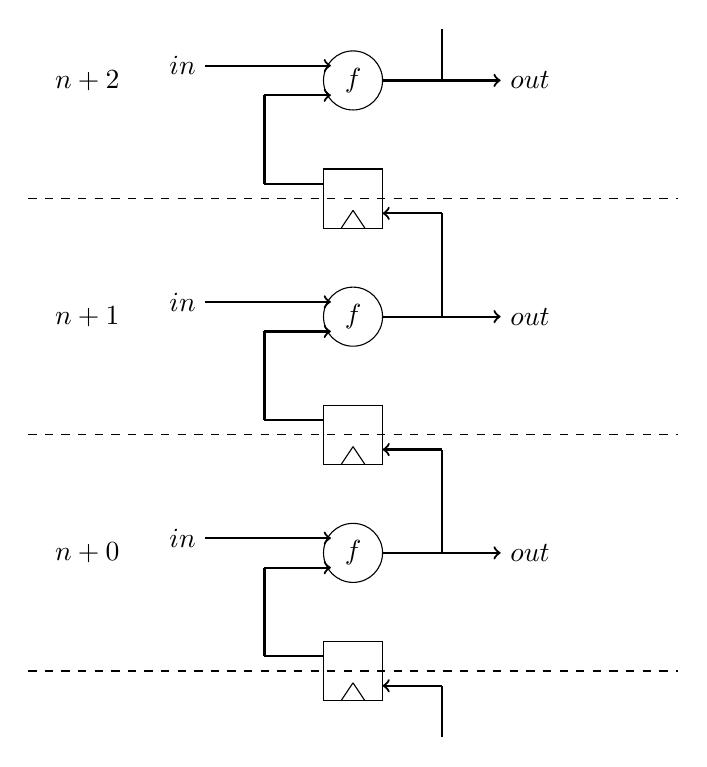
\begin{tikzpicture}[scale=0.75]
\foreach \c/\t in {0/0,4/1,8/2} {

    \draw (1,2.5+\c) node { $n+\t$ };
    \draw[dashed] (0,0.5+\c) -- (11,0.5+\c);

    \draw[thick,-] (5,0.75+\c) -- (4,0.75+\c);
    \draw[thick,-] (4,0.75+\c) -- (4,2.25+\c);
    \draw[thick,->] (4,2.25+\c) -- (5.125,2.25+\c);
    \draw[thick,->] (3,2.75+\c) -- (5.125,2.75+\c);


    \draw[thick,->] (7,0.25+\c) -- (6,0.25+\c);
    \draw[thick,-] (7,2.5+\c) -- (7,3.375+\c);
    \draw[thick,-] (7,-0.625+\c) -- (7,0.25+\c);
    \draw[thick,->] (7,2.5+\c) -- (8,2.5+\c);
    \draw[thick,-] (6,2.5+\c) -- (7,2.5+\c);
    \draw (8,2.5+\c) node[right] { $out$ };
    \draw (3,2.75+\c) node[left] { $in$ };

    \draw (5.5,2.5+\c) node { $f$ };
    \draw (5.5,2.5+\c) circle (0.5);

    \draw (5,0+\c) rectangle (6,1+\c);
    \draw (5.3,0+\c) -- (5.5,0.3+\c);
    \draw (5.7,0+\c) -- (5.5,0.3+\c);
}
\end{tikzpicture}
%\caption{Temporal perspective of feedback} \label{fig:chronfeedback}
\end{figure}

Like mentioned before, this is not really the interface we want to use, as it exposes the \textit{internal} interface of the function to the external world.
Even though we define a certain input as coming from the past there are two issues:
\begin{itemize}
 \item We have not yet bound input to output, we have merely defined that we want \textit{some} input from the past.
 \item We cannot combine this function with other functions.
\end{itemize}

To use a more realistic example in further discussion we use the \ensuremath{\Varid{sum}} function as defined in code snippet \ref{code:chronsum}.
\begin{texexptitled}[text only,float]{Definition for a specific multiply and add}{code:mul32add}
\begin{hscode}\SaveRestoreHook
\column{B}{@{}>{\hspre}l<{\hspost}@{}}%
\column{E}{@{}>{\hspre}l<{\hspost}@{}}%
\>[B]{}\Varid{sum}\mathbin{::}\Conid{Int}\langle\Varid{n}\rangle\to \Conid{Int}\langle\Varid{n}\mathbin{-}\mathrm{1}\rangle\to \Conid{Int}\langle\Varid{n}\rangle{}\<[E]%
\\
\>[B]{}\Varid{sum}\;\Varid{input}\;\Varid{feedback}\mathrel{=}\Varid{input}\mathbin{+}\Varid{feedback}{}\<[E]%
\ColumnHook
\end{hscode}\resethooks
%\caption{Chronological function definition of sum using feedback} \label{code:chronsum}
\end{texexptitled}

The two issues from before can be solved by introducing a primitive, shown in code snippet \ref{code:transpart}, which turns the partial recursive function in a total recursive function.
From figure \ref{fig:chronfeedback} we can see that \ensuremath{\Varid{sum}} is actually an infinite chain of dependencies.
In order to evaluate feedback in a finite amount of time we need a method to give an initial value.

\begin{texexptitled}[text only,float]{Definition for a specific multiply and add}{code:mul32add}
\begin{hscode}\SaveRestoreHook
\column{B}{@{}>{\hspre}l<{\hspost}@{}}%
\column{E}{@{}>{\hspre}l<{\hspost}@{}}%
\>[B]{}\leftarrow\mathbin{::}(\Varid{a}\langle\Varid{n}\rangle\to \Varid{a}\langle\Varid{n}\mathbin{-}\Varid{k}\rangle\to \Varid{a}\langle\Varid{n}\rangle)\to (\Varid{a}\langle\Varid{n}\rangle\to \Varid{a}\langle\Varid{n}\rangle){}\<[E]%
\ColumnHook
\end{hscode}\resethooks
%\caption{Primitive for transforming partially recursive functions} \label{code:transpart}
\end{texexptitled}
We can then use it on the sum example:
\begin{texexptitled}[text only,float]{Definition for a specific multiply and add}{code:mul32add}
\begin{hscode}\SaveRestoreHook
\column{B}{@{}>{\hspre}l<{\hspost}@{}}%
\column{5}{@{}>{\hspre}l<{\hspost}@{}}%
\column{17}{@{}>{\hspre}l<{\hspost}@{}}%
\column{E}{@{}>{\hspre}l<{\hspost}@{}}%
\>[B]{}\Varid{sum}\mathbin{::}\Conid{Int}\langle\Varid{n}\rangle\to \Conid{Int}\langle\Varid{n}\rangle{}\<[E]%
\\
\>[B]{}\Varid{sum}\;\Varid{x}\mathrel{=}\Varid{sum'}\;\Varid{x}\leftarrow(\mathrm{0}\;\Conid{Int}\mathbin{::<}\mathrm{0}\rangle){}\<[E]%
\\
\>[B]{}\hsindent{5}{}\<[5]%
\>[5]{}\mathbf{where}\;{}\<[17]%
\>[17]{}\Varid{sum'}\mathbin{::}\Conid{Int}\langle\Varid{n}\rangle\to \Conid{Int}\langle\Varid{n}\mathbin{-}\mathrm{1}\rangle\to \Conid{Int}\langle\Varid{n}\rangle{}\<[E]%
\\
\>[17]{}\Varid{sum'}\;\Varid{input}\;\Varid{feedback}\mathrel{=}\Varid{input}\mathbin{+}\Varid{feedback}{}\<[E]%
\ColumnHook
\end{hscode}\resethooks
%\caption{Total recursive function definition of sum} \label{code:totalchronsum}
\end{texexptitled}
What is clear from the example is that the initial state is bound to a specific moment in time. 
This introduces a constraint, namely that this function is only defined for $n >= 0$.
Through this constraint it is clear that we are \textit{restricting} the possible inputs to this partially recursive function and as a result turning it into a total recursive function; i.e. a function for which we can determine whether it will halt.

Lets say we want to define a component which computes the running average of two numbers. 
We can do this in various ways, shown in both figure \ref{code:chronavg1} and \ref{code:chronavg2}.
The major difference is the use of adts \todo{ref} to help with readability.
First, we average the two inputs and pass the result to the \ensuremath{\Varid{average'}} component which includes a feedback structure to store the needed state.
Of course, there may be smarter ways to do this, but for the purpose of illustration this example works well enough.
\begin{texexptitled}[text only,float]{Definition for a specific multiply and add}{code:mul32add}
\begin{hscode}\SaveRestoreHook
\column{B}{@{}>{\hspre}l<{\hspost}@{}}%
\column{5}{@{}>{\hspre}l<{\hspost}@{}}%
\column{9}{@{}>{\hspre}l<{\hspost}@{}}%
\column{E}{@{}>{\hspre}l<{\hspost}@{}}%
\>[B]{}\mbox{\onelinecomment  Average two numbers and create a running average of the result}{}\<[E]%
\\
\>[B]{}\Varid{average}\mathbin{::}\Conid{Int}\langle\Varid{n}\rangle\to \Conid{Int}\langle\Varid{n}\rangle\to \Conid{Int}\langle\Varid{n}\rangle{}\<[E]%
\\
\>[B]{}\Varid{average}\;\Varid{x}\;\Varid{y}\mathrel{=}{}\<[E]%
\\
\>[B]{}\hsindent{5}{}\<[5]%
\>[5]{}\mathbf{let}\;\Varid{z}\mathrel{=}(\Varid{x}\mathbin{+}\Varid{y})\mathbin{/}\mathrm{2}{}\<[E]%
\\
\>[B]{}\hsindent{5}{}\<[5]%
\>[5]{}\mathbf{in}\;{}\<[9]%
\>[9]{}\Varid{average'}\;\Varid{z}\leftarrow\mathrm{0}\langle\mathrm{0}\rangle{}\<[E]%
\ColumnHook
\end{hscode}\resethooks
\begin{hscode}\SaveRestoreHook
\column{B}{@{}>{\hspre}l<{\hspost}@{}}%
\column{17}{@{}>{\hspre}l<{\hspost}@{}}%
\column{21}{@{}>{\hspre}c<{\hspost}@{}}%
\column{21E}{@{}l@{}}%
\column{25}{@{}>{\hspre}l<{\hspost}@{}}%
\column{33}{@{}>{\hspre}l<{\hspost}@{}}%
\column{37}{@{}>{\hspre}l<{\hspost}@{}}%
\column{E}{@{}>{\hspre}l<{\hspost}@{}}%
\>[B]{}\Varid{average'}\mathbin{::}{}\<[17]%
\>[17]{}\Conid{Int}\langle\Varid{n}\rangle{}\<[E]%
\\
\>[17]{}\to (\Conid{Int}\langle\Varid{n}\mathbin{-}\mathrm{1}\rangle,\Conid{Int}\langle\Varid{n}\mathbin{-}\mathrm{1}\rangle,\Conid{Int}\langle\Varid{n}\mathbin{-}\mathrm{1}\rangle)\to {}\<[E]%
\\
\>[17]{}(\Conid{Int}\langle\Varid{n}\rangle,\Conid{Int}\langle\Varid{n}\rangle,\Conid{Int}\langle\Varid{n}\rangle){}\<[E]%
\\
\>[B]{}\Varid{average'}\;\Varid{x}\;(\Varid{t},\Varid{c},\Varid{a}){}\<[21]%
\>[21]{}\mathrel{=}{}\<[21E]%
\>[25]{}\mathbf{let}\;{}\<[33]%
\>[33]{}\Varid{t'}{}\<[37]%
\>[37]{}\mathrel{=}\Varid{t}\mathbin{+}\Varid{x}{}\<[E]%
\\
\>[33]{}\Varid{c'}{}\<[37]%
\>[37]{}\mathrel{=}\Varid{c}\mathbin{+}\mathrm{1}{}\<[E]%
\\
\>[33]{}\Varid{a'}{}\<[37]%
\>[37]{}\mathrel{=}\Varid{t'}\mathbin{/}\Varid{c'}{}\<[E]%
\\
\>[25]{}\mathbf{in}\;(\Varid{t'},\Varid{c'},\Varid{a'}){}\<[E]%
\ColumnHook
\end{hscode}\resethooks
%\caption{Averaging numbers from two streams of values} \label{code:chronavg1}
\end{texexptitled}
\begin{texexptitled}[text only,float]{Definition for a specific multiply and add}{code:mul32add}
\begin{hscode}\SaveRestoreHook
\column{B}{@{}>{\hspre}l<{\hspost}@{}}%
\column{17}{@{}>{\hspre}l<{\hspost}@{}}%
\column{33}{@{}>{\hspre}c<{\hspost}@{}}%
\column{33E}{@{}l@{}}%
\column{41}{@{}>{\hspre}l<{\hspost}@{}}%
\column{49}{@{}>{\hspre}l<{\hspost}@{}}%
\column{58}{@{}>{\hspre}l<{\hspost}@{}}%
\column{E}{@{}>{\hspre}l<{\hspost}@{}}%
\>[B]{}\mathbf{data}\;\Conid{Average}{}\<[17]%
\>[17]{}\mathrel{=}\Conid{Average}\;\Conid{Int}\;\Conid{Int}\;\Conid{Int}{}\<[E]%
\\[\blanklineskip]%
\>[B]{}\Varid{average'}\mathbin{::}\Conid{Int}\langle\Varid{n}\rangle\to \Conid{Average}\langle\Varid{n}\mathbin{-}\mathrm{1}\rangle\to \Conid{Average}\langle\Varid{n}\rangle{}\<[E]%
\\
\>[B]{}\Varid{average'}\;\Varid{x}\;(\Conid{Average}\;\Varid{t}\;\Varid{c}\;\anonymous ){}\<[33]%
\>[33]{}\mathrel{=}{}\<[33E]%
\>[41]{}\mathbf{let}\;{}\<[49]%
\>[49]{}\Varid{t'}{}\<[58]%
\>[58]{}\mathrel{=}\Varid{t}\mathbin{+}\Varid{x}{}\<[E]%
\\
\>[49]{}\Varid{c'}{}\<[58]%
\>[58]{}\mathrel{=}\Varid{c}\mathbin{+}\mathrm{1}{}\<[E]%
\\
\>[49]{}\Varid{a'}{}\<[58]%
\>[58]{}\mathrel{=}\Varid{t'}\mathbin{/}\Varid{c'}{}\<[E]%
\\
\>[41]{}\mathbf{in}\;{}\<[49]%
\>[49]{}\Conid{Average}\;\Varid{t'}\;\Varid{c'}\;\Varid{a'}{}\<[E]%
\ColumnHook
\end{hscode}\resethooks
\begin{hscode}\SaveRestoreHook
\column{B}{@{}>{\hspre}l<{\hspost}@{}}%
\column{5}{@{}>{\hspre}l<{\hspost}@{}}%
\column{9}{@{}>{\hspre}l<{\hspost}@{}}%
\column{E}{@{}>{\hspre}l<{\hspost}@{}}%
\>[B]{}\Varid{average}\mathbin{::}\Conid{Int}\langle\Varid{n}\rangle\to \Conid{Int}\langle\Varid{n}\rangle\to \Conid{Average}\langle\Varid{n}\rangle{}\<[E]%
\\
\>[B]{}\Varid{average}\;\Varid{x}\;\Varid{y}\mathrel{=}{}\<[E]%
\\
\>[B]{}\hsindent{5}{}\<[5]%
\>[5]{}\mathbf{let}\;\Varid{z}\mathrel{=}(\Varid{x}\mathbin{+}\Varid{y})\mathbin{/}\mathrm{2}{}\<[E]%
\\
\>[B]{}\hsindent{5}{}\<[5]%
\>[5]{}\mathbf{in}\;{}\<[9]%
\>[9]{}\Varid{average'}\;\Varid{z}\leftarrow(\Conid{Average}\;\mathrm{0}\;\mathrm{0}\;\mathrm{0}\mathbin{::}\Conid{Average}\langle\mathrm{0}\rangle){}\<[E]%
\ColumnHook
\end{hscode}\resethooks
%\caption{Averaging numbers from two streams of values using adts} \label{code:chronavg2}
\end{texexptitled}
Of course not every element of the \ensuremath{\Conid{Average}} structure is something we want to use, so we can transform the output:
\begin{texexptitled}[text only,float]{Definition for a specific multiply and add}{code:mul32add}
\begin{hscode}\SaveRestoreHook
\column{B}{@{}>{\hspre}l<{\hspost}@{}}%
\column{E}{@{}>{\hspre}l<{\hspost}@{}}%
\>[B]{}\Varid{averageC}\mathbin{::}\Conid{Int}\langle\Varid{n}\rangle\to \Conid{Int}\langle\Varid{n}\rangle\to \Conid{Int}\langle\Varid{n}\rangle{}\<[E]%
\\
\>[B]{}\Varid{averageC}\mathrel{=}(\lambda(\Conid{Average}\;\Varid{x}\;\Varid{y}\;\Varid{z})\to \Varid{z})\mathbin{\circ}\Varid{average}{}\<[E]%
\ColumnHook
\end{hscode}\resethooks
%\caption{Selecting a specific output from |Average|} \label{code:chronavgsel}
\end{texexptitled}

\subsection{Composition and Higher Order Functions}
Function composition in functional languages can be defined in various ways.
One way of function composition is simply using another function in the definition of a function.
For regular functions composition is fairly straightforward, but to make our chronological functions work we need to clarify what effect this has on timing constraints.
To show the basic concept of time variables when composing chronological functions we can define a simple component, shown in figure \ref{code:chronmulacc}.
\begin{texexptitled}[text only,float]{Definition for a specific multiply and add}{code:mul32add}
\begin{hscode}\SaveRestoreHook
\column{B}{@{}>{\hspre}l<{\hspost}@{}}%
\column{E}{@{}>{\hspre}l<{\hspost}@{}}%
\>[B]{}\Varid{mulacc}\mathbin{::}\Conid{Int}\langle\Varid{n}\rangle\to \Conid{Int}\langle\Varid{n}\rangle\to \Conid{Int}\langle\Varid{n}\mathbin{+}\mathrm{2}\rangle\to \Conid{Int}\langle\Varid{n}\mathbin{+}\mathrm{2}\rangle{}\<[E]%
\\
\>[B]{}\Varid{mulacc}\;\Varid{x}\;\Varid{y}\;\Varid{z}\mathrel{=}\Varid{x}\mathbin{*}\Varid{y}\mathbin{+}\Varid{z}{}\<[E]%
\ColumnHook
\end{hscode}\resethooks
%\caption{A single multiply-accumulate computation} \label{code:chronmulacc}
\end{texexptitled}
For this component we might know the multiplication part takes a few cycles to complete\footnote{For simplicity this component is considered a streaming component.}, something for which the third parameter is not needed.
From this definition we can also deduce that the addition operation is combinational, as no extra delay is introduced.
Moreover, if we have all values available at the same time we should be able to silently add delays to the third argument, since it is early enough for the computation to work.
Lets say we have an operation \ensuremath{\lambda \Varid{x}\to \Varid{x}\mathbin{*}\Varid{x}\mathbin{+}\Varid{x}\mathbin{+}\mathrm{42}}\footnote{This is simply x*(x+1)+42}, then we can simply define it as a function that uses the definition of \ensuremath{\Varid{mulacc}}:
\begin{texexptitled}[text only,float]{Definition for a specific multiply and add}{code:mul32add}
\begin{hscode}\SaveRestoreHook
\column{B}{@{}>{\hspre}l<{\hspost}@{}}%
\column{E}{@{}>{\hspre}l<{\hspost}@{}}%
\>[B]{}\Varid{squarePlusOne}\;\Varid{x}\mathrel{=}\mathrm{42}\mathbin{+}(\Varid{mulacc}\;\Varid{x}\;\Varid{x}\;\Varid{x}){}\<[E]%
\ColumnHook
\end{hscode}\resethooks
%\caption{Using the multiply accumulate function to define a squaring function} \label{code:chronsquare}
\end{texexptitled}
, without even needing timing information as this can be inferred from the environment, though for documentation purposes we can actually add these.

As mentioned earlier, we can use function composition in two distinct ways.
Another way is the \ensuremath{\mathbin{\circ}} operator, which is already used in Haskell, as shown in code snippet \ref{code:composition}.
\begin{texexptitled}[text only,float]{Definition for a specific multiply and add}{code:mul32add}
\begin{hscode}\SaveRestoreHook
\column{B}{@{}>{\hspre}l<{\hspost}@{}}%
\column{E}{@{}>{\hspre}l<{\hspost}@{}}%
\>[B]{}(\mathbin{\circ})\mathbin{::}(\Varid{b}\to \Varid{c})\to (\Varid{a}\to \Varid{b})\to \Varid{a}\to \Varid{c}{}\<[E]%
\ColumnHook
\end{hscode}\resethooks
%\caption{Function composition as in Haskell} \label{code:composition}
\end{texexptitled}

The timed equivalent, shown in code snippet \ref{code:chroncomp}, would be much the same, except it will silently add constraints. \todo{Need to show which constraints}
\begin{texexptitled}[text only,float]{Definition for a specific multiply and add}{code:mul32add}
\begin{hscode}\SaveRestoreHook
\column{B}{@{}>{\hspre}l<{\hspost}@{}}%
\column{9}{@{}>{\hspre}l<{\hspost}@{}}%
\column{E}{@{}>{\hspre}l<{\hspost}@{}}%
\>[B]{}(\mathbin{\circ}){}\<[9]%
\>[9]{}\mathbin{::}(\Varid{b}\langle\Varid{n}\rangle\to \Varid{c}\langle\Varid{m}\rangle){}\<[E]%
\\
\>[9]{}\to (\Varid{a}\langle\Varid{p}\rangle\to \Varid{b}\langle\Varid{q}\rangle){}\<[E]%
\\
\>[9]{}\to \Varid{a}\langle\Varid{r}\rangle\to \Varid{c}\langle\Varid{s}\rangle{}\<[E]%
\ColumnHook
\end{hscode}\resethooks
%\caption{Chronological function composition} \label{code:composition}
\end{texexptitled}
The constraints may be inferred from the environment, so the actual constraints do not have to be given when defining the function.
The \ensuremath{\mathbin{\circ}} operator has a structural representation, shown in figure \ref{fig:composition}.
Since we have multiple forms of composition we will refer to \ensuremath{\mathbin{\circ}} as \textit{serial composition}.
\begin{figure}
\centering
\footnotesize
\begin{tikzpicture}[scale=0.4]
\draw (0,0) rectangle +(6,4);
\draw (10,0) rectangle +(6,4);
\draw[->,thick] (-4,2) -- (0,2);
\draw[->,thick] (6,2) -- (10,2);
\draw[->,thick] (16,2) -- (20,2);
\draw (3,2) node { $foo$ };
\draw (13,2) node { $bar$ };

\draw (-4,2) node[left] { $a$ };
\draw (8,2) node[above] { $b$ };
\draw (20,2) node[right] { $c$ };

\end{tikzpicture}
%\caption{Serial composition} \label{fig:composition}
\end{figure}

Aside from serial composition, we can also compose functions in parallel, with the composed functions interacting. 
The signature for this operator is shown in code snippet \ref{code:parcomp}.\todo{add constraints}
\begin{texexptitled}[text only,float]{Definition for a specific multiply and add}{code:mul32add}
\begin{hscode}\SaveRestoreHook
\column{B}{@{}>{\hspre}l<{\hspost}@{}}%
\column{9}{@{}>{\hspre}l<{\hspost}@{}}%
\column{E}{@{}>{\hspre}l<{\hspost}@{}}%
\>[B]{}(\langle || \rangle){}\<[9]%
\>[9]{}\mathbin{::}(\Varid{c}\langle\Varid{n}\rangle\to \Varid{b}\langle\Varid{m}\rangle\to (\Varid{a}\langle\Varid{p}\rangle,\Varid{d}\langle\Varid{q}\rangle)){}\<[E]%
\\
\>[9]{}\to (\Varid{a}\langle\Varid{r}\rangle\to \Varid{b}\langle\Varid{s}\rangle){}\<[E]%
\\
\>[9]{}\to \Varid{c}\langle\Varid{t}\rangle\to \Varid{d}\langle\Varid{u}\rangle{}\<[E]%
\ColumnHook
\end{hscode}\resethooks
%\caption{Parallel composition with interaction}\label{code:parcomp}
\end{texexptitled}
This  makes the composition \ensuremath{\Varid{foo}\;\langle || \rangle\;\Varid{bar}} look like:
\begin{figure}[H]
\centering
\footnotesize
\begin{tikzpicture}[scale=0.4]
\draw[->,thick] (2,4) -- (2,8);
\draw[->,thick] (4,8) -- (4,4);
\draw (0,0) rectangle +(6,4);
\draw (0,8) rectangle +(6,4);
\draw[->,thick] (-4,2) -- (0,2);
\draw[->,thick] (6,2) -- (10,2);
\draw (3,2) node { $foo$ };
\draw (3,10) node { $bar$ };

\draw (-4,2) node[left] { $c$ };
\draw (10,2) node[right] { $d$ };
\draw (2,6) node[left] { $a$ };
\draw (4,6) node[right] { $b$ };

\end{tikzpicture}
%\caption{Parallel composition with interaction} \label{fig:parcomp}
\end{figure}

\subsection{Types, Algebraic Datatypes and Contracts}

\section{Choice}
\todo[inline]{Choice might actually not be this hard...}
Choice is a harder concept to deal with when dealing with chronological functions. 
The problem we are facing with is the possibility there is a choice between components which introduce different latencies.
For now, we do not support choice for different clock frequencies.

The fundamental problem is not so much the choice itself.
We can formulate a way to bind the scrutinee\todo{add glos} to a certain delay, as in code snippet \ref{code:timeclass}, but even then we have not actually solved the entire problem.
\begin{texexptitled}[text only,float]{Definition for a specific multiply and add}{code:mul32add}
\begin{hscode}\SaveRestoreHook
\column{B}{@{}>{\hspre}l<{\hspost}@{}}%
\column{5}{@{}>{\hspre}l<{\hspost}@{}}%
\column{11}{@{}>{\hspre}l<{\hspost}@{}}%
\column{E}{@{}>{\hspre}l<{\hspost}@{}}%
\>[B]{}\Conid{Timeclass}\;\Conid{MyControl}\;\Conid{Bool}\langle\Varid{t}\rangle\mathbf{where}{}\<[E]%
\\
\>[B]{}\hsindent{5}{}\<[5]%
\>[5]{}\Conid{True}{}\<[11]%
\>[11]{}\mathbin{::}\psi. n.\;\Conid{Bool}\langle\Varid{n}\mathbin{+}\mathrm{1}\rangle{}\<[E]%
\\
\>[B]{}\hsindent{5}{}\<[5]%
\>[5]{}\Conid{False}\mathbin{::}\psi. n.\;\Conid{Bool}\langle\Varid{n}\mathbin{+}\mathrm{2}\rangle{}\<[E]%
\ColumnHook
\end{hscode}\resethooks
\begin{hscode}\SaveRestoreHook
\column{B}{@{}>{\hspre}l<{\hspost}@{}}%
\column{5}{@{}>{\hspre}l<{\hspost}@{}}%
\column{9}{@{}>{\hspre}l<{\hspost}@{}}%
\column{17}{@{}>{\hspre}l<{\hspost}@{}}%
\column{E}{@{}>{\hspre}l<{\hspost}@{}}%
\>[B]{}\Varid{myChoice}\mathbin{::}\Conid{Int}\langle\Varid{n}\rangle\to \Conid{Bool}\langle\Varid{n}\rangle\to \Conid{Int}\langle\Varid{t}\rangle\mid \Conid{MyControl}\;\Conid{Bool}\langle\Varid{t}\rangle{}\<[E]%
\\
\>[B]{}\Varid{myChoice}\;\Varid{x}\;\Varid{choice}\mathrel{=}{}\<[E]%
\\
\>[B]{}\hsindent{5}{}\<[5]%
\>[5]{}\mathbf{case}\;\Varid{choice}\;\mathbf{of}{}\<[E]%
\\
\>[5]{}\hsindent{4}{}\<[9]%
\>[9]{}\Conid{True}{}\<[17]%
\>[17]{}\to \mathbin{...}{}\<[E]%
\\
\>[5]{}\hsindent{4}{}\<[9]%
\>[9]{}\Conid{False}{}\<[17]%
\>[17]{}\to \mathbin{...}{}\<[E]%
\ColumnHook
\end{hscode}\resethooks
%\caption{TimeClass definition for choice}
\end{texexptitled}
Whenever we compose...

\section{Syntactic Sugar}
\subsection{Sampling input}
One extension of the concepts used before is the ability to sample a input.
For instance, if we have a certain algorithm which needs 3 consequitive frames of data from a source, but needs to apply a certain transformation to the data.
If this transformation depends purely on the input from the 3 frames of data we can model this as a sub-stream of elements:
\begin{texexp}{text only}
\begin{hscode}\SaveRestoreHook
\column{B}{@{}>{\hspre}l<{\hspost}@{}}%
\column{E}{@{}>{\hspre}l<{\hspost}@{}}%
\>[B]{}\Varid{sample}\mathbin{::}\Conid{Frame}\langle\Varid{n},\Varid{n}\mathbin{+}\mathrm{1},\Varid{n}\mathbin{+}\mathrm{2}\rangle\to \Conid{ProcessedFrame}\langle\Varid{n}\mathbin{+}\mathrm{3}\rangle{}\<[E]%
\\
\>[B]{}\Varid{sample}\langle\Varid{x},\Varid{y},\Varid{z}\rangle\mathrel{=}\Varid{processFrames}\;\Varid{x}\;\Varid{y}\;\Varid{z}{}\<[E]%
\ColumnHook
\end{hscode}\resethooks
\end{texexp}
This is assuming we can process all frames in 1 clockcycle, given all the data in advance.
If we have a more complex algorithm which can handle some tasks on a per-frame basis, then we can simply introduce them, assuming the total delay is no more than described in the function signature:
\begin{texexp}{text only}
\begin{hscode}\SaveRestoreHook
\column{B}{@{}>{\hspre}l<{\hspost}@{}}%
\column{5}{@{}>{\hspre}l<{\hspost}@{}}%
\column{13}{@{}>{\hspre}l<{\hspost}@{}}%
\column{E}{@{}>{\hspre}l<{\hspost}@{}}%
\>[B]{}\Varid{sample}\mathbin{::}\Conid{Frame}\langle\Varid{n},\Varid{n}\mathbin{+}\mathrm{1},\Varid{n}\mathbin{+}\mathrm{2}\rangle\to \Conid{ProcessedFrame}\langle\Varid{n}\mathbin{+}\mathrm{3}\rangle{}\<[E]%
\\
\>[B]{}\Varid{sample}\langle\Varid{x},\Varid{y},\Varid{z}\rangle\mathrel{=}\Varid{processFrames}\;\Varid{xy}\;\Varid{z}{}\<[E]%
\\
\>[B]{}\hsindent{5}{}\<[5]%
\>[5]{}\mathbf{where}\;{}\<[13]%
\>[13]{}\Varid{x'}\mathrel{=}\Varid{processFrame}\;\Varid{x}{}\<[E]%
\\
\>[13]{}\Varid{y'}\mathrel{=}\Varid{processFrame}\;\Varid{y}{}\<[E]%
\\
\>[13]{}\Varid{xy}\mathrel{=}\Varid{extractCommon}\;\Varid{x'}\;\Varid{y'}{}\<[E]%
\ColumnHook
\end{hscode}\resethooks
\end{texexp}

